


\tikzset{every picture/.style={line width=0.75pt}} %set default line width to 0.75pt        

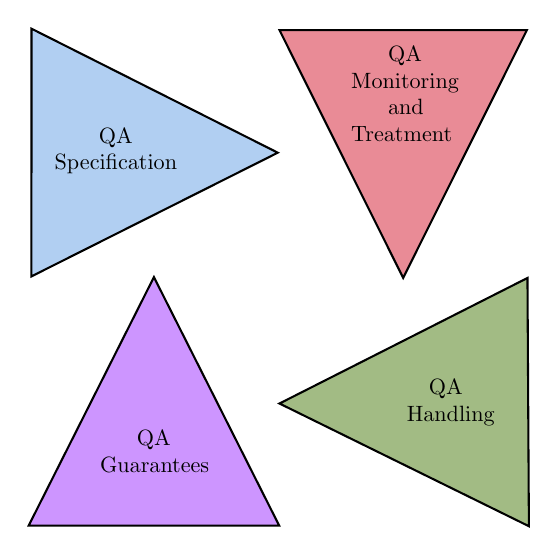
\begin{tikzpicture}[x=0.75pt,y=0.75pt,yscale=-1,xscale=1]
%uncomment if require: \path (0,262); %set diagram left start at 0, and has height of 262

%Flowchart: Extract [id:dp5939698678534469] 
\draw  [fill={rgb, 255:red, 74; green, 144; blue, 226 }  ,fill opacity=0.43 ] (131,70.03) -- (12.3,129.64) -- (12.36,10.3) -- cycle ;
%Flowchart: Merge [id:dp5767066916635984] 
\draw  [fill={rgb, 255:red, 208; green, 2; blue, 27 }  ,fill opacity=0.46 ] (131.83,11) -- (251,11) -- (191.42,130.33) -- cycle ;
%Flowchart: Extract [id:dp6600751137454604] 
\draw  [fill={rgb, 255:red, 65; green, 117; blue, 5 }  ,fill opacity=0.49 ] (131.82,190.88) -- (251.3,130.39) -- (251.99,249.99) -- cycle ;
%Flowchart: Extract [id:dp5337732612018415] 
\draw  [fill={rgb, 255:red, 144; green, 19; blue, 254 }  ,fill opacity=0.45 ] (71.33,130) -- (131.67,249.67) -- (11,249.67) -- cycle ;

% Text Node
\draw (53,69.33) node [scale=0.8] [align=left] { \ \ \ \ \ \ QA \\Specification};
% Text Node
\draw (192.33,41.67) node [scale=0.8] [align=left] { \ \ \ \ \ QA\\Monitoring \\ \ \ \ \ \ and \\Treatment};
% Text Node
\draw (214.33,190.33) node [scale=0.8] [align=left] { \ \ \ QA \\Handling};
% Text Node
\draw (71.67,214) node [scale=0.8] [align=left] { \ \ \ \ \ QA\\Guarantees};


\end{tikzpicture}
